\section{Methods}\label{sec:Methods}

Our general approach is illustrated in Figure~\ref{fig:systemBlockDiagram}. For visualizations that are open to instrumentation, gaze coordinates provided by eye-trackers can be mapped to visual objects displayed on the screen automatically and in real-time, since the computer generated visual content and its layout is known during rendering.  Specifically, a visualization instrumented with our approach will not only draw visual primitives on the screen (e.g., nodes in a graph), but will also inform a viewed-object detection algorithm about where such primitives are drawn and their shape. The viewed-object detection algorithm uses this information to map 2D gaze coordinates to visualization objects rendered on the screen. Should the visualization be transformed (e.g., zoomed, panned), its content altered (e.g., filtering), or individual visualization components moved (e.g., dragging a node), the detection module is informed about these changes as soon as the visualization is redrawn and will map subsequent gaze samples to the new visual layout. 

\begin{figure}[htb]
  \centering
  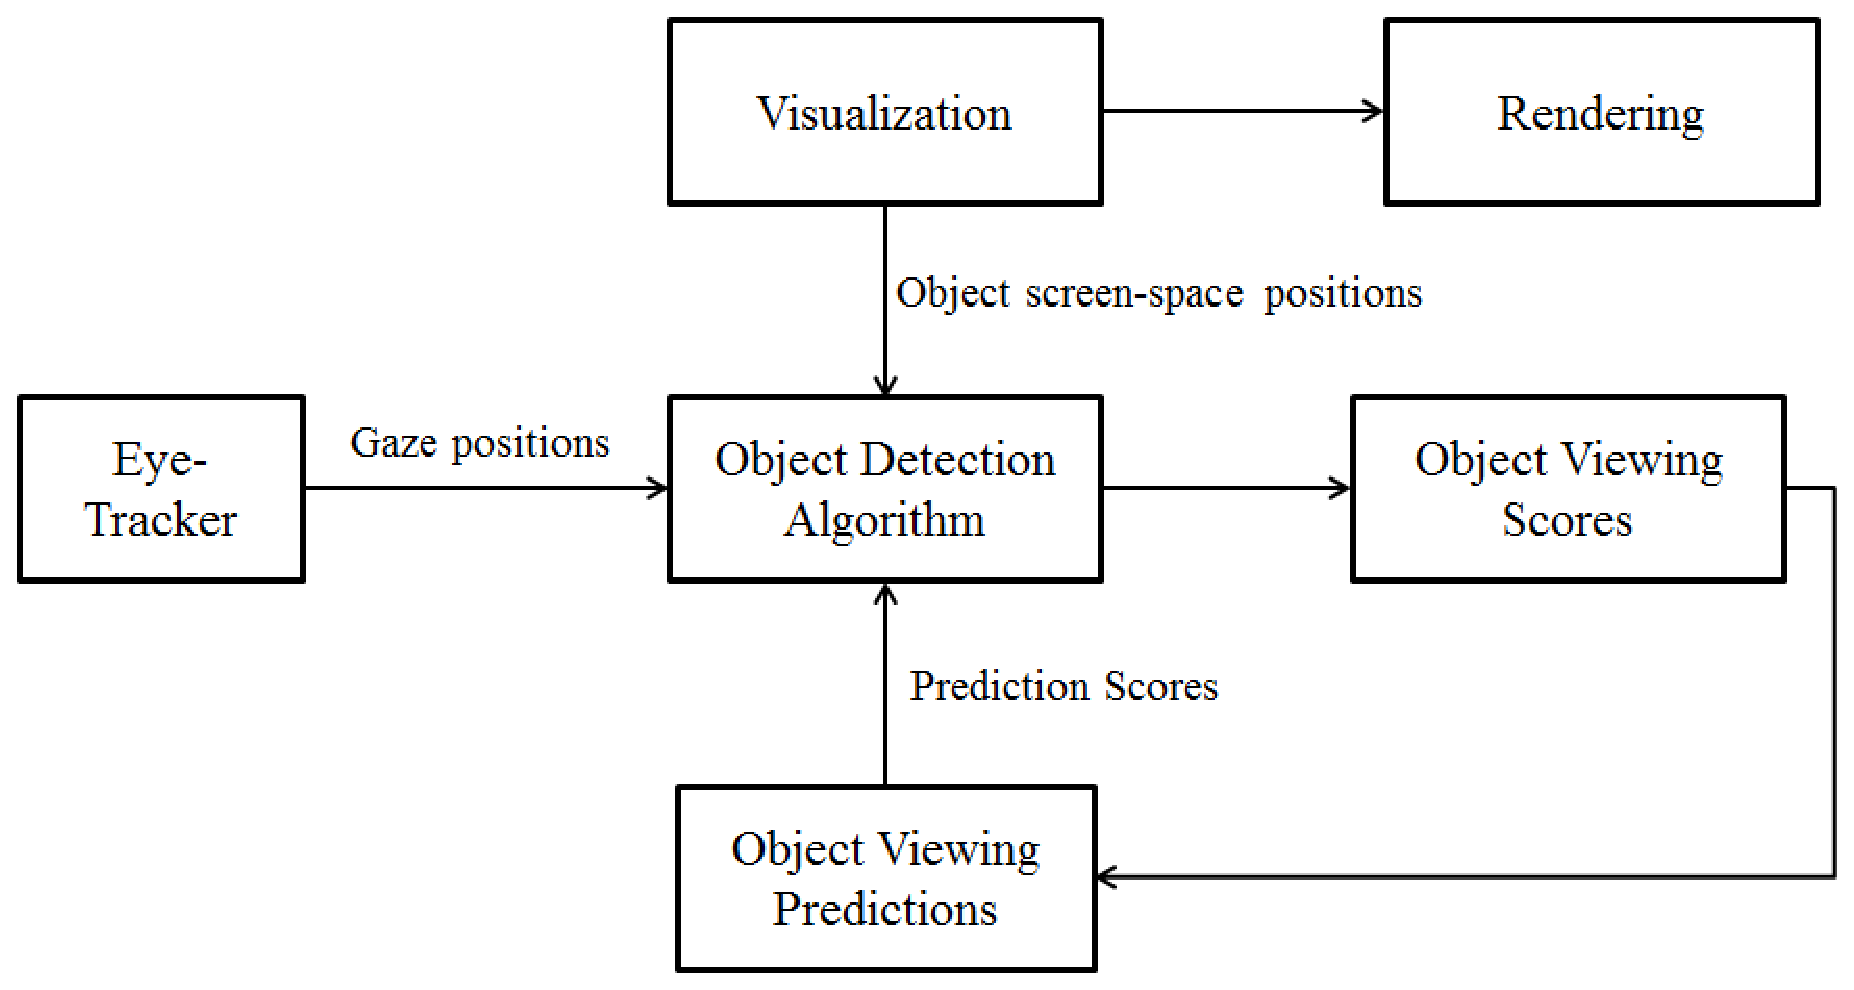
\includegraphics[width=\linewidth]{images/systemBlockDiagram.eps}
  \caption{Real-time detection of viewed objects in generative visualizations.}
	\label{fig:systemBlockDiagram}
\end{figure}

Next, we describe an effective algorithm for mapping gaze samples to objects that users are viewing. As shown in Figure~\ref{fig:systemBlockDiagram}, we will assume that gaze samples have already been transformed from screen space into model space. As such, the basic input of our algorithm is a stream of gaze samples in model space, and a list of visual primitives drawn on the screen, together with their shape and position. The algorithm outputs a stream of viewed visualization and data primitives (e.g., nodes, labels) in real-time, as users are viewing them in the instrumented visualization. Of course, our approach is limited in that it cannot be applied to already rendered images or videos. 

We will describe our algorithm incrementally in the following three sections, starting from a na\"{\i}ve approach that simply draws AOIs dynamically around visualization objects, to an `intelligent' one that detects objects more accurately by using knowledge about how specific visualizations may be typically used.  A comparative evaluation of these three object detection algorithms is presented in Section~\ref{sec:EvalResults}.

\subsection{Algorithms for viewed object detection in data visualizations}
\subsubsection{AOI-based viewed object detection}
\label{sec:AOIBasedViewedObjectDetection}
A na\"{\i}ve viewed object detection approach is to treat object shapes as dynamic AOIs and determine that the viewed object is that with the most recent fixation landing in its AOI. This is a natural first try at detecting viewed visual objects from gaze data, given that manually drawn AOIs are typically used in the same manner in offline eye-tracking data analysis, and that the similar concept of objects of interest (OOIs) has been proposed already by Stellmach et al.~\cite{stellmach20103d} for generative 3D content.

The problem with this approach is that for highly granular visualization content, such as individual nodes or labels, users often fixate in the vicinity of the object rather than on the object itself. We demonstrate and quantify this observation in our evaluation section. A potential solution to this problem could be to make object AOIs slightly larger than the objects themselves. However, larger AOIs may lead to AOI overlap in cluttered visualizations. Ultimately, the problem lies with an inability to determine with absolute certainty what a user is looking at, and is described in more detail in the next section.

\subsubsection{A probabilistic approach to viewed object detection}
\label{sec:ProbabilisticObjectDetection}
Unlike mouse input, eye-tracking can only indicate a small screen region that a user is fixating, rather than a particular pixel. Typically, such a region is about one inch in diameter, though specific values depend on the user's distance to the monitor, and is determined by how human vision works. As such, we argue that it is generally impossible to tell with absolute certainty which object a user is viewing, if the user is fixating in the vicinity of multiple close objects (Figure~\ref{fig:discreminateFig4}(a)). This is not a significant problem for traditional AOI analyses, which generally use large AOIs. However, our goal is to detect the viewing of granular visual content, such as network nodes or glyphs, in cluttered visualizations. 

\begin{figure}[htb]
  \centering
  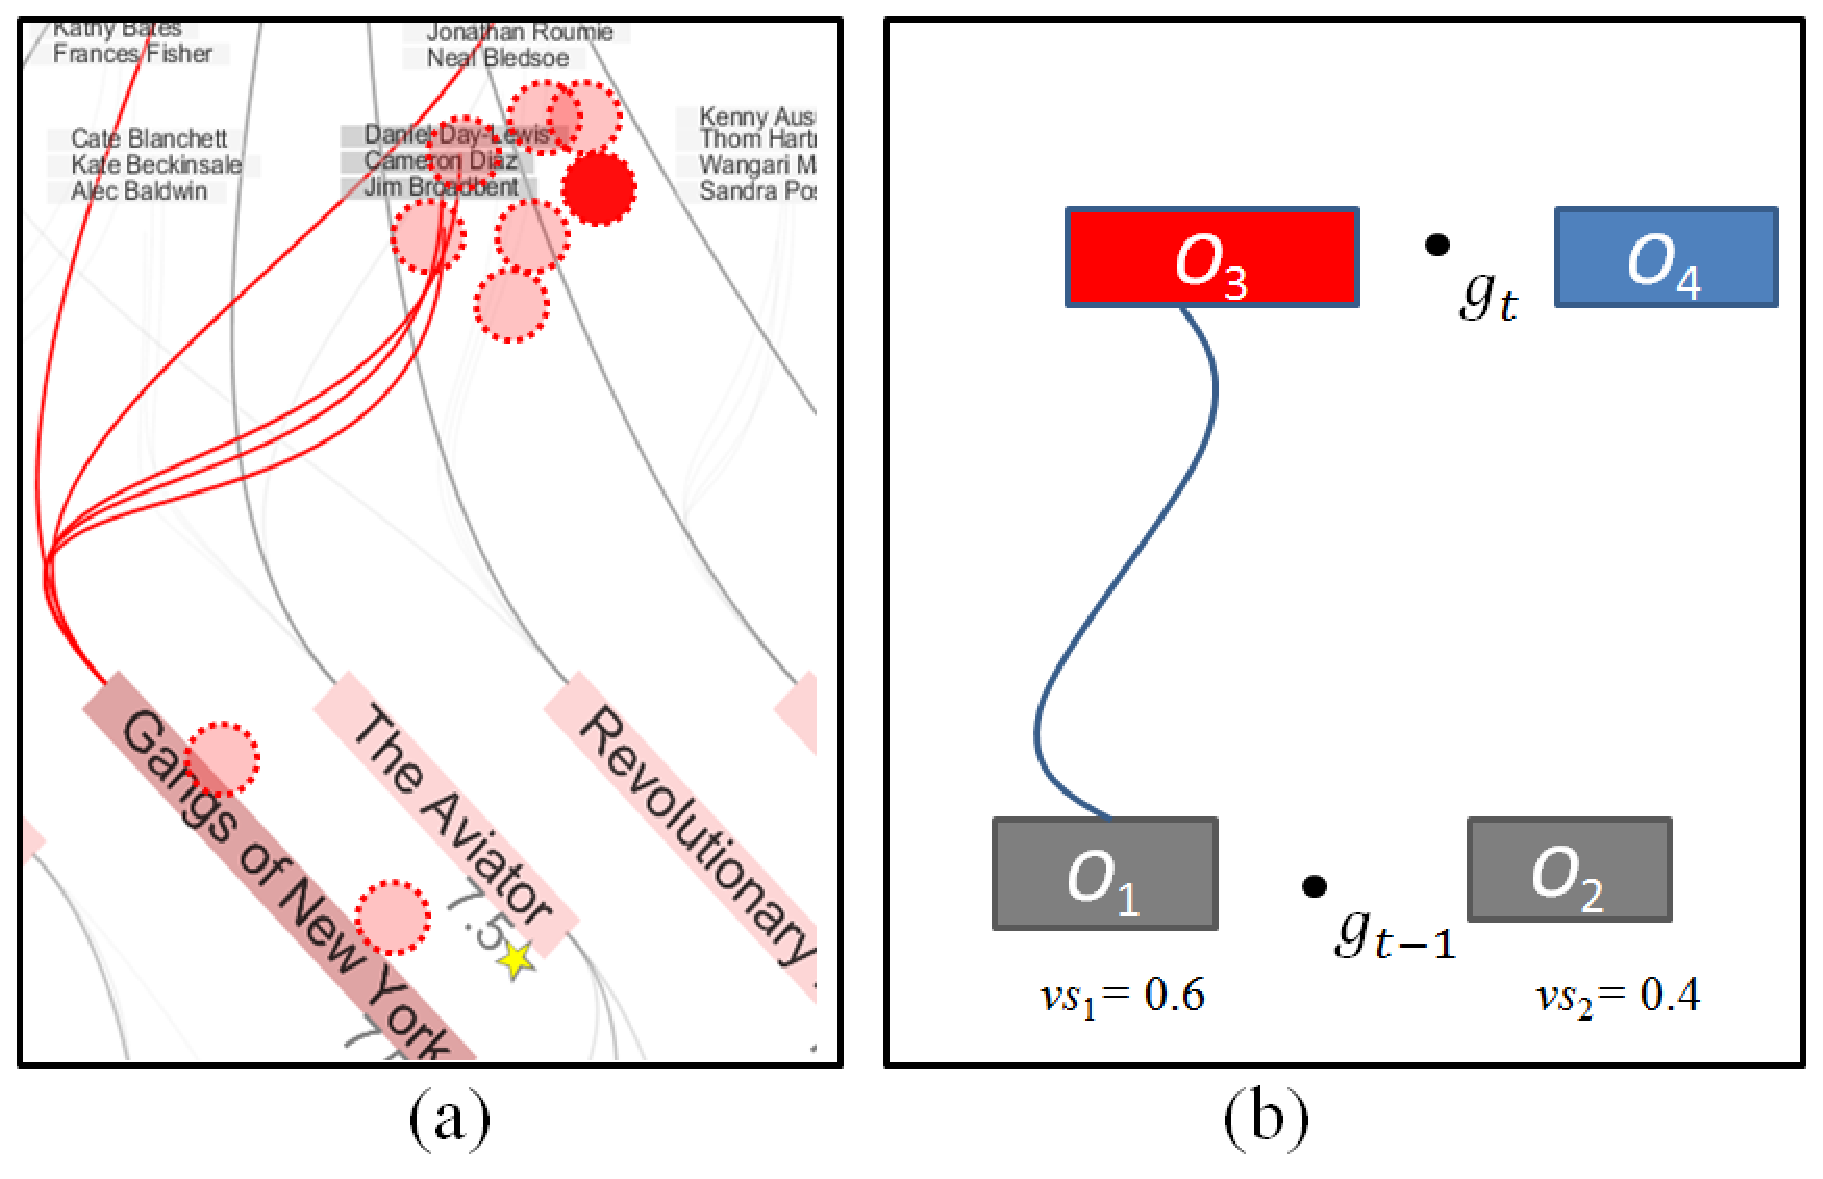
\includegraphics[width=\linewidth]{images/discreminateFig4.eps}
  \caption{(a) A real visualization example in which a user fixates in the vicinity of multiple close object groups (red dot). (b) ``Intelligent gaze interpretation'': even though the latest gaze sample falls equidistantly between visual objects O3 and O4, we suspect that O3 is the more likely viewing target given that (i) it is highlighted, and (ii) it is connected to O1, which is likely to have been the object that the user viewed previously ($vs_1=0.6 > vs_2 = 0.4$. }
	\label{fig:discreminateFig4}
\end{figure}

As such, we advocate for a fuzzy interpretation of gaze data and detecting likelihoods that objects are viewed rather than certainties. To this end, we can compute object gazes scores $gs$ that range between zero- the object is not viewed, and one- the object is certainly viewed as shown in Figure~\ref{fig:gazeScoreFig3} and Formula~\ref{eq:GS}. The region of radius $R$ used in the formula is analogue to the user's foveated region, and as such needs to be constant in screen space. Thus, if the view is zoomed in or out, $R$ needs to be scaled accordingly in model space to remain constant in screen space.  A more detailed discussion about choosing an appropriate $R$ is given in the discussion section [REMINDER]. Finally, we mention that similar approaches were used by Salvucci et al.~\cite{salvucci2000intelligent} and Okoe et al.~\cite{okoe2014gaze}.
Finally, we note that the object scores ($gs$) do not directly equate to probabilities. The distinction is important because it implies that our implementation can detect two objects as being viewed simultaneously ($gs_1 = 1$ and $gs_2=1$). We think this is appropriate since a person can in fact visually register multiple objects at the same time, and in fact even think of them as a unit using the process of mental information chunking.


\subsubsection{An intelligent algorithm for viewed object detection in data visualization}
\label{sec:MehthodsIntelligentAlgorithm}
Salvucci and Anderson described the concept of ``intelligent gaze interpretation'' in the context of a gaze-activated interface ~\cite{salvucci2000intelligent}. Their method achieved better accuracy in detecting which interface control a user is gazing at, by integrating both the proximity of the gaze to the control, and the likelihood that the control would be the target of a gaze-interaction in the interfaces' current state and context of use. Formally, their algorithm identifies the most likely currently viewed item $i_{viewed}$ by solving 

\begin{equation*}
i_{viewed} = \displaystyle \argmax_{i\in I}[Pr(g|i)\cdot Pr(i)]
\end{equation*}

, where $Pr(g|i)$ is the probability of producing a gaze at location $g$ given the intention of viewing item $i$, and $Pr(i)$ is the prior probability of an item $i$  being the target of a gaze-interaction. In Salvucci and Anderson's proof of concept implementation these prior probabilities were based on assumptions about how an interface might be used and were hardcoded into the system.  


We adapt Salvucci and Anderson's paradigm to increase the accuracy of determining which particular object a user might be viewing when a gaze-sample is registered in the vicinity of multiple objects, such as in Figure~\ref{fig:discreminateFig4}(a). For example, we may assume that in a network visualization, a user who has just viewed a node $n$ will more likely view one of $n$'s neighbors than a random other node, perhaps especially if the user previously highlighted node $n$ and its outgoing edges.  As we will show in our evaluation section, such assumptions hold for the visualization we tested. 

We illustrate this scenario in Figure~\ref{fig:discreminateFig4}(b): four visual objects ($O_{1\ldots 4}$), two of which are connected ($O_1$ and $O_3$), and one of which is highlighted ($O_3$), are shown on the screen. A new gaze sample registers between $O_3$ and $O_4$. Intuitively, it is more likely that $O_3$ was viewed since it is highlighted. Moreover, if we knew that $O_1$ was viewed just before the current moment, and, as described above we assume that users generally view neighboring nodes together, then this likelihood becomes even stronger.  
Formally, we compute a viewing score $vs$ of object $i$ at time $t$ ($vs(i,t)$) by weighing the gaze score $gs(i,t)$ described in Section~\ref{sec:ProbabilisticObjectDetection} by a prediction score $ps(i,t)$ that object $i$ is a viewing target at time $t$ (Formula~\ref{eq:ps}). This prediction score is computed based on the likelihood that the object is viewed given the current state of the visualization (e.g., the object is highlighted), and the likelihood that it is viewed if some other specific object (e.g.,  a node's neighbor) was viewed just before it. Those two components are formalized by the  $\alpha$ score and $\beta$ score in Formula~\ref{eq:beta}.

\begin{figure}[htb]
  \centering
  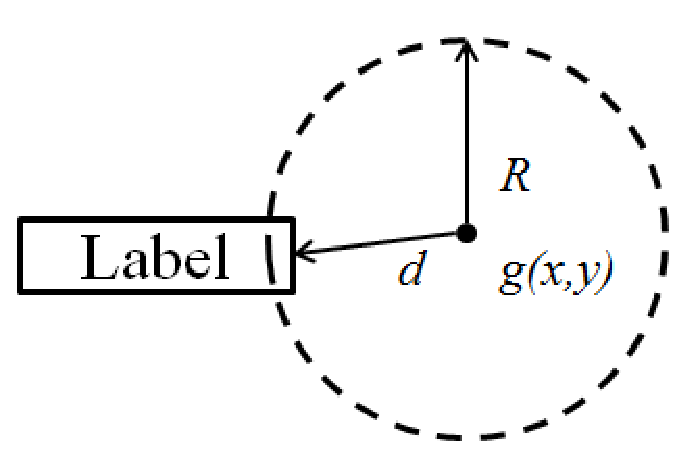
\includegraphics[width=0.5\linewidth]{images/gazeScoreFig3.eps}
  \caption{Calculating a gaze score $gs$ for a given object and a gaze sample landing nearby, where $d$ is the distance from the object to the gaze sample, and $R$ is the radius of the user's foveated region. }
	\label{fig:gazeScoreFig3}
\end{figure}
%Formula 1
\begin{equation}
gs_{i,t} = 1 - \min (1, (\frac{d}{R}))
\label{eq:GS}
\end{equation}

%Formula 2
\begin{equation}
vs_{i,t} = gs_{i,t} \times ps_{i,t}
\label{eq:VS}
\end{equation}

%Formula 3
\begin{equation}
ps_{i,t} = \alpha_{i,t} \times \beta_{i,t}
\label{eq:ps}
\end{equation}

%Formula 4
\begin{equation}
\beta_{i,t} = \frac{\displaystyle\sum_{j} {vs_{j,t-1} \times T(j,i)}}{\displaystyle\sum_{j} vs_{j,t-1}} \text{ , where  } \parbox{15em}{$0\geq i \geq n$ and $gs_{i,t} > 0$\\ $0\geq j \geq n$ and $gs_{j,t} = 0$}
\label{eq:beta}
\end{equation}


First, we will assume $\alpha$ is given as an input to our algorithm. Concrete examples of what $\alpha$ could be linked to are whether an object is highlighted (larger alpha) or not, whether an object is part of a group of objects recently queried by the user, or whether an object is known to be of particular interest to the users' current workflow. 
Second, we will compute $\beta$ based on a viewing transition function between object:  $T(i,j)$ gives the likelihood that object $j$ is viewed after object $i$ is viewed. We will again assume that $T(i,j)$ is given as input to our algorithm. Concrete examples of what $T(i,j)$ could be linked to are whether objects $i$ and $j$ are connected by an edge, or whether they are part of a cluster. To compute $\beta$, we could consider $\beta_{j,t} = T(i,j)$ but that would involve knowing $i$, the previously viewed object, with absolute certainty. This is problematic because unlike Salvucci and Anderson, we wish to avoid making an unequivocal determination of which precise item was viewed at any given time, and instead aim to consider all objects with non-zero viewing scores as potentially viewed. In other words, we don't always know for sure what the previously viewed element was. As illustrated in Figure~\ref{fig:discreminateFig4}(b), $O_1$'s previous viewing score ($vs_{1,t-1}=0.6$), is just slightly larger than $O_2$'s viewing score ($vs_{2,t-1}=0.4$), and thus an absolute choice of $O_1$ over $O_2$ as previously viewed element would be rather arbitrary. 

To avoid this, we use a weighted average of transition probabilities from $O_1$ and $O_2$ to $O_3$ and $O_4$, using the previous view scores of $O_1$ and $O_2$ as weights.  More generally, $\beta_{i,t}$ is computed as shown in Formula~\ref{eq:beta}. In essence, the previously viewed objects $O_1$ and $O_2$ act as referees with varying degrees of influence in a competition between $O_3$ and $O_4$. This analogy provides an intuition for an additional important guideline: an object should not referee a competition that it is part of. For example, using $O_3$ as a previous element in a competition between itself and $O_4$ would result in an open feedback-loop and should be avoided. This restriction is reflected in Formula~\ref{eq:beta}.  Finally, the algorithm pseudocode is provided in Algorithm~\ref{alg:ObjectDetection}.

\begin{algorithm}
\caption{Viewed Object Detection Algorithm}
\label{alg:ObjectDetection}
\begin{algorithmic}[1]
\State \textbf{Inputs: } 
\Statex $O_{i, \ldots, n}$= tracked visualization objects (shapes, positions)
\Statex $g(x,y) = $ gaze sample in model space (time $t$)
\Statex $\alpha_{i, \ldots, n} = $ view weights ($\alpha_{i, \ldots, n} \in [0,1]$)
\Statex $T(i,j) = $ viewing transition function ($T(i,j) \in [0,1]$)
\State \textbf{Outputs:}
\Statex $vs_{i,t} = $ momentary viewing scores of all objects ($i = 1, \ldots, n$). 
\For{$i \gets 1 \text{ to } n$}
	\State Compute $gs_{i,t}$	using Formula~\ref{eq:GS}
\EndFor
\State $max \gets 0$
\For{$i \gets 1 \text{ to } n$}
	\If{$gs_{i,t} > 0$} \label{algLine:PredictionScoreLines}
		\State $\beta_{i,t} \gets \frac{vs_{j,t-1} \times T(i,j)}{vs_{j,t-1}}$
		\State $ps'_{i,t} \gets \alpha_{i,t} \times \beta_{i,t}$
		\If{$ps'_{i,t} > max$}
			\State $max \gets ps'_{i,t}$
		\EndIf
	\EndIf
\EndFor
\For{$i \gets 1 \text{ to } n$}
	\State $vs_{i,t} \gets gs_{i,t} \times \frac{ps'_{i,t}}{max} $
\EndFor
\end{algorithmic}
\end{algorithm}

Finally, we note two more factors. First, to optimize for speed, we only compute prediction scores for objects with non-zero gazes (Algorithm~\ref{alg:ObjectDetection}, line~\ref{algLine:PredictionScoreLines}). Second, in our implementation we compute viewing scores for every gaze sample, rather than every fixation. We believe that doing so leads to results that are less dependent on how fixations are computed and more robust. Since our eye-tracker's sampling rate is $60$Hz, the scores $vs_{i, t-1}$ indicate objects that were `viewed' just $15$ms ago, an interval much shorter than the time it takes for people to shift their attention to a new object. As such, instead of using the raw $vs_{j,t-1}$ score, we use an average of the last several viewing scores. For all practical purposes, the term $vs_{j,t-1}$ should be replaced in the previous formulas by $ \sum_{k=1}^{k=20}{vs_{j,t-1}}$.  However, our algorithm can take as input fixations rather than individual gaze samples, in which case this step would not be necessary. 
%(Sayeed, make sure that all indeces and terms here are up to date and make sense in the context of this section).

{\bf Performance analysis:} The algorithm needs to swift through all tracked elements ($n$) to find those in the proximity of a gaze sample or fixation ($k_t$). Then, to compute the term $\beta$ for each of the $k_t$ potentially viewed elements, the algorithm will iterate over $k_{t-1}$ objects with non-zero viewing scores from the previous iteration. So the complexity of the algorithm is 
\begin{equation*}
T(n) = O( n+ \max (k_{t-1}, k_t)) 
\label{eq:RuntimeComplexity}
\end{equation*}
%Is this correct?


\subsection{Instrumenting a concrete visualization}

\begin{figure*}[htb]
  \centering
  \includegraphics[width=0.75\linewidth]{images/pivotpaths.eps}
  \caption{PivotPaths visualization of IMDB data. Movies are displayed in the center of the screen, actors at the top, and directors and genres share the bottom space. Actors, directors, and genres associated to movies are connected through curves. Users can highlight objects and their connected neighbors by hovering over them.}
	\label{fig:pivotpaths}
\end{figure*}
We have used the previously described principles to instrument Doerk's interactive PivotPaths visualization of multifaceted data~\cite{dork2012pivotpaths}, which we linked to the popular internet movie database (IMDB). Shown in Figure~\ref{fig:pivotpaths}, the visualization renders movies in the center of the screen, actors on top, and genres and directors at the bottom. Actors, directors, and genres are connected by curves to the movies they associate with, and are larger, and their connections more salient, if they are associated with multiple movies. Actors, genres, and directors are colored distinctively, which is particular important for genres and directors since they occupy the same visual space. Such views are created in response to users' searches for specific movies, actors, and directors, and show data that is most relevant to the search. As shown in Figure~\ref{fig:pivotpaths}, users can hover over visual elements to highlight them and their connections. Users can also click on visual elements to transition the view to one centered on the select element. Finally, users can freely zoom and pan the visualization. 

We opted to instrument this particular visualization for three reasons. First, it is highly interactive and would thus be significantly difficult to analyze using manual gaze data analysis. Second, it contains visual metaphors, graphic primitives, and interactions typical of a wide range of visualizations. Third, we used the popular IMDB data source to leverage the familiarity of our prospective user-study subjects to it.  

To apply the previously described instrumentation algorithm to this visualization, we had to choose appropriate values for the $\alpha$ and $\beta$ factors defined in Formulas~\ref{eq:beta}. To this end, we made informal assumptions about how the visualization may be used, a method also employed by Salvucci~\cite{salvucci2000intelligent}. For instance, we assumed that transitions between connected items would occur more often than between unconnected items. We also assumed that elements that are hovered or highlighted are more likely to be viewed than those that are not. We translated these assumptions into specific weights, as exemplified in Table in~\ref{tab:Transition2}. As we will show in our evaluation section~\ref{sec:Evaluation}, these assumptions hold for the pivot paths visualization and the nine subjects that used it in our study.

A more principled way to determine typical viewing patterns and sequences in a specific visualization is to run a pilot study and collect data using the algorithm described in section~\ref{sec:ProbabilisticObjectDetection}, which does not require the $\alpha$ and $\beta$ inputs. Such preliminary data could be used to determine typical usage patterns and help refine viewed object detection by informing the choice of appropriate $\alpha$ and $\beta$ factors. We show how such an analysis can be done in section~\ref{sec:Evaluation}. 

\begin{table}[htbp]
	\centering
		\begin{tabular}{|l|c|}
			\hline
			 \multicolumn{2}{|c|}{Assumed visual and transition weights} \\ \hline
			Movie to unconnected actor & 0.3\\\hline
			Movie to connected actor & 1\\\hline
			Movie to unconnected genre & 0.2\\\hline
			Movie to connected genre & 0.8\\\hline
			Movie to unconnected director & 0.3\\\hline
			Movie to connected director & 1\\\hline
			Any object hovered & 1\\\hline
			Any object not hovered & 0.5\\
			\hline			
		\end{tabular}
	\caption{Transition probabilities in our instrumented visualization (assumed).}
	\label{tab:Transition2}
\end{table}



Finally, as part of instrumentation, our system collected application screen shots, interactive events (e.g., hovering, zooming, panning), raw gaze samples captured at a rate of $60$Hz, and visual elements with non-zero viewing scores computed at the same rate of $60$Hz. For each viewed element we recorded the type (i.e., movie, actor, director, genre), its label, its gaze score ($gs$), its prediction score ($ps$), and the aggregated viewing score ($vs$). All recorded data was time stamped. 
